%
% Complete documentation on the extended LaTeX markup used for Insight
% documentation is available in ``Documenting Insight'', which is part
% of the standard documentation for Insight.  It may be found online
% at:
%
%     http://www.itk.org/

\documentclass{InsightArticle}


%%%%%%%%%%%%%%%%%%%%%%%%%%%%%%%%%%%%%%%%%%%%%%%%%%%%%%%%%%%%%%%%%%
%
%  hyperref should be the last package to be loaded.
%
%%%%%%%%%%%%%%%%%%%%%%%%%%%%%%%%%%%%%%%%%%%%%%%%%%%%%%%%%%%%%%%%%%
\usepackage[dvips,
bookmarks,
bookmarksopen,
backref,
colorlinks,linkcolor={blue},citecolor={blue},urlcolor={blue},
]{hyperref}
% to be able to use options in graphics
\usepackage{graphicx}
% for pseudo code
\usepackage{listings}
% subfigures
\usepackage{subfigure}


%  This is a template for Papers to the Insight Journal. 
%  It is comparable to a technical report format.

% The title should be descriptive enough for people to be able to find
% the relevant document. 
\title{Histogram-based thresholding - some missing methods}

% 
% NOTE: This is the last number of the "handle" URL that 
% The Insight Journal assigns to your paper as part of the
% submission process. Please replace the number "1338" with
% the actual handle number that you get assigned.
%
\newcommand{\IJhandlerIDnumber}{}

% Increment the release number whenever significant changes are made.
% The author and/or editor can define 'significant' however they like.
\release{0.00}

% At minimum, give your name and an email address.  You can include a
% snail-mail address if you like.
\author{Richard Beare{$^1$} {\small{and}} Ga\"etan Lehmann{$^2$}}
\authoraddress{{$^1$}Department of Medicine, Monash University, Australia.\\ 
{$^2$}INRA, UMR 1198; ENVA; CNRS, FRE 2857, Biologie du D\'eveloppement et 
Reproduction, Jouy en Josas, F-78350, France}



\begin{document}


%
% Add hyperlink to the web location and license of the paper.
% The argument of this command is the handler identifier given
% by the Insight Journal to this paper.
% 
\IJhandlefooter{\IJhandlerIDnumber}{3279}

\maketitle

\ifhtml
\chapter*{Front Matter\label{front}}
\fi


\begin{abstract}
\noindent
% The abstract should be a paragraph or two long, and describe the
% scope of the document.
Using intensity histograms to estimate image thresholds is a long
established practice in image processing and image analysis and a wide
variety of techniques have been developed. Different techniques are
appropriate for different intensity distributions. This article
implements a number of standard techniques not currently available in
ITK.
\end{abstract}

\IJhandlenote{\IJhandlerIDnumber}

\tableofcontents

\section{Introduction}
This contribution includes classes for threshold estimation using the
following methods: Huang\cite{huang1995image},
Intermodes and Minimum\cite{prewitt1965analysis}, IsoData\cite{ridler1978picture},
Li\cite{li1993minimum,li1998iterative}, MaxEntropy\cite{kapur1985new},
KittlerIllingworth\cite{kittler1986minimum},
Moments\cite{tsai1985moment}, Yen\cite{yen1995new},
RenyiEntropy\cite{kapur1985new},
Shanbhag\cite{shanbhag1994utilization} and
Triangle\cite{zack1977automatic}.

All classes are largely derived from the AutoThresh
\cite{LandiniImageJ} package for ImageJ. Parts of the brief outline below are
taken from the presentation associated with the
HistThresh\cite{HistThreshMatlab} matlab toolbox, which was also a
source of information for the AutoThresh package. The exception is the
triangle method, that was written before discovery of the AutoThresh
packge and before this project got slightly out of hand.

These classes have been included in ITK 4 and are implented using the
histogram framework. Methods for setting number of histogram bins and 

\section{Thresholding algorithms}
\subsection{Huang}
{\em itkHuangThresholdImageFilter} implements Huang's fuzzy
thresholding using Shannon's entropy
function\cite{huang1995image}. The measure of fuzziness represents the
difference between the original image and its binary version. For a
given threshold level the fuzzy membership function for a pixel is defined by the
absolute difference between the pixel gray level and the average gray
level of the region to which it belongs, with a larger difference
leading to a smaller membership value. The optimal threshold is
the value that minimizes the fuzziness, as defined by Shannon's
entropy function, applied to the fuzzy membership functions.

\subsection{Intermodes}
{\em itkIntermodesThresholdImageFilter} implements the methods
described in \cite{prewitt1965analysis}. The histogram is iteratively
smoothed until only 2 peaks remain. In one variant the threshold is
the midpoint of the two peaks, while in the other it is the minimum
point between the peaks. The two variants are selected using the {\em
  UseIntermodeOff} method. Not good for histograms with very unequal
peaks.
\subsection{IsoData}
{\em itkIsoDataThresholdImageFilter} implements Ridler and Calvard's
\cite{ridler1978picture} isodata method. 
Computes average of voxels below initial threshold and above initial
threshold. Threshold is set to the average of the two. Repeat until
the threshold is larger than the average of the brightness of the two regions.

\subsection{Li}
 {\em itkLiThresholdImageFilter} implements Li's minimum cross entropy
 method\cite{li1993minimum,li1998iterative}. This method selects a
 threshold that minimizes the cross entropy between original and
 thresholded images.
\subsection{MaxEntropy}
 {\em itkMaxEntropyThresholdImageFilter} implements the method
 described in \cite{kapur1985new}, which chooses a threshold such that the entropies of distributions above and
below threshold are maximised. One of several entropy-based approaches.
\subsection{RenyiEntropy}
{\em itkRenyiEntropyThresholdImageFilter} Similar to MaxEntropy, but using a different entropy measure\cite{kapur1985new}.

\subsection{KittlerIllingworth}
 {\em itkKittlerIllingworthThresholdImageFilter} implements the minimum
error thresholding method\cite{kittler1986minimum}. A threshold is
selected that minimizes the number of misclassifications between the
two normal distributions with the given means, variances and
proportions. This method assumes a Gaussian mixture model, similar to
the Otsu method.
\subsection{Moments}
{\em itkMomentsThresholdImageFilter} implements Tsai's moment
preserving approach \cite{tsai1985moment} that chooses a threshold such that the binary image has the same first three moments as the grey level image.
\subsection{Yen}
{\em itkYenThresholdImageFilter} implements thresholding based on a
maximum correlation criterion \cite{yen1995new} as a more
computationally efficient alternative to entropy measures.

\subsection{Shanbhag}
 {\em itkShanbhagThresholdImageFilter} implements Shanbhag's
 extenstion of the Kapur method\cite{shanbhag1994utilization} that
 includes a distance from the threshold in the entropy measure.

\subsection{Triangle}
{\em itkTriangleThresholdImageFilter} implements a variant of \cite{zack1977automatic}
The triangle method constructs a line between the histogram peak and
the farthest end of the histogram. The threshold is the point of
maximum distance between the line and the histogram. This
implementation uses robust (default is 1\% and 99\%) estimation of histogram ends.

\section{Results}
A cropped and smoothed version of the BrainProtonDensitySlice image is used to demonstrate the results. Smoothing has been applied to avoid the gaps in the histogram and cropping has been applied to remove a peak at 0 caused by padding in the original. This is a slightly challenging image to threshold as there are 3 classes, but the two brighter ones overlap. The mode-based approaches, results in Figure \ref{fig:bpdthreshA}, select thresholds between the darkest (background) class and the foreground, thus merging the two foreground classes. Some of the entropy measures, shown in Figure \ref{fig:bpdthreshB}, attempt to split the two foreground classes, with varying degrees of success. The thresholds are shown on the histogram in Figure \ref{fig:thresh}.

\begin{figure}[htbp]
\centering
\includegraphics[angle=180,totalheight=5cm]{BrainProtonDensitySliceBorder20}
\caption{The input image.\label{fig:bpd}}
\end{figure}

\begin{figure}[htbp]
\centering
\subfigure[Kittler Illingworth]{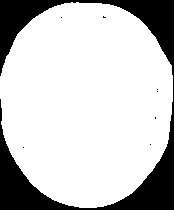
\includegraphics[angle=180,totalheight=5cm]{outKittlerIllingworth}}
\subfigure[Intermode]{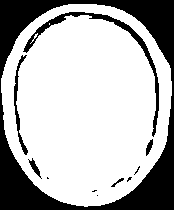
\includegraphics[angle=180,totalheight=5cm]{outIntermodes}}
\subfigure[Intermode - minimum]{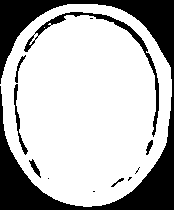
\includegraphics[angle=180,totalheight=5cm]{outMinimum}}

\subfigure[IsoData]{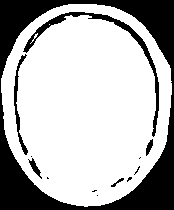
\includegraphics[angle=180,totalheight=5cm]{outIsoData}}
\subfigure[Monents]{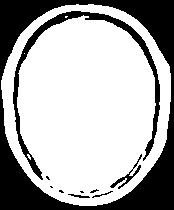
\includegraphics[angle=180,totalheight=5cm]{outMoments}}
\subfigure[Triangle]{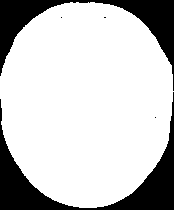
\includegraphics[angle=180,totalheight=5cm]{outTriangle}}
\caption{Thresholded images.\label{fig:bpdthreshA}}
\end{figure}

\begin{figure}[htbp]
\centering
\subfigure[Huang]{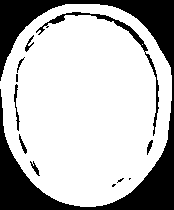
\includegraphics[angle=180,totalheight=5cm]{outHuang}}
\subfigure[Li]{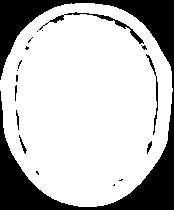
\includegraphics[angle=180,totalheight=5cm]{outLi}}
\subfigure[Maximum Entropy]{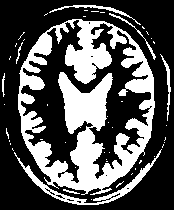
\includegraphics[angle=180,totalheight=5cm]{outMaxEntropy}}

\subfigure[Renyi Entropy]{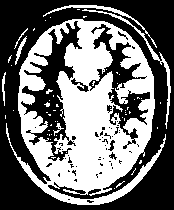
\includegraphics[angle=180,totalheight=5cm]{outRenyiEntropy}}
\subfigure[Yen]{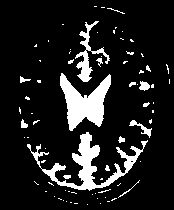
\includegraphics[angle=180,totalheight=5cm]{outYen}}
\subfigure[Shanbhag]{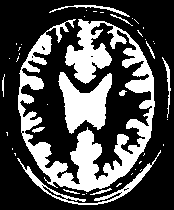
\includegraphics[angle=180,totalheight=5cm]{outShanbhag}}
\caption{Thresholded images.\label{fig:bpdthreshB}}
\end{figure}

\begin{figure}[htbp]
\centering
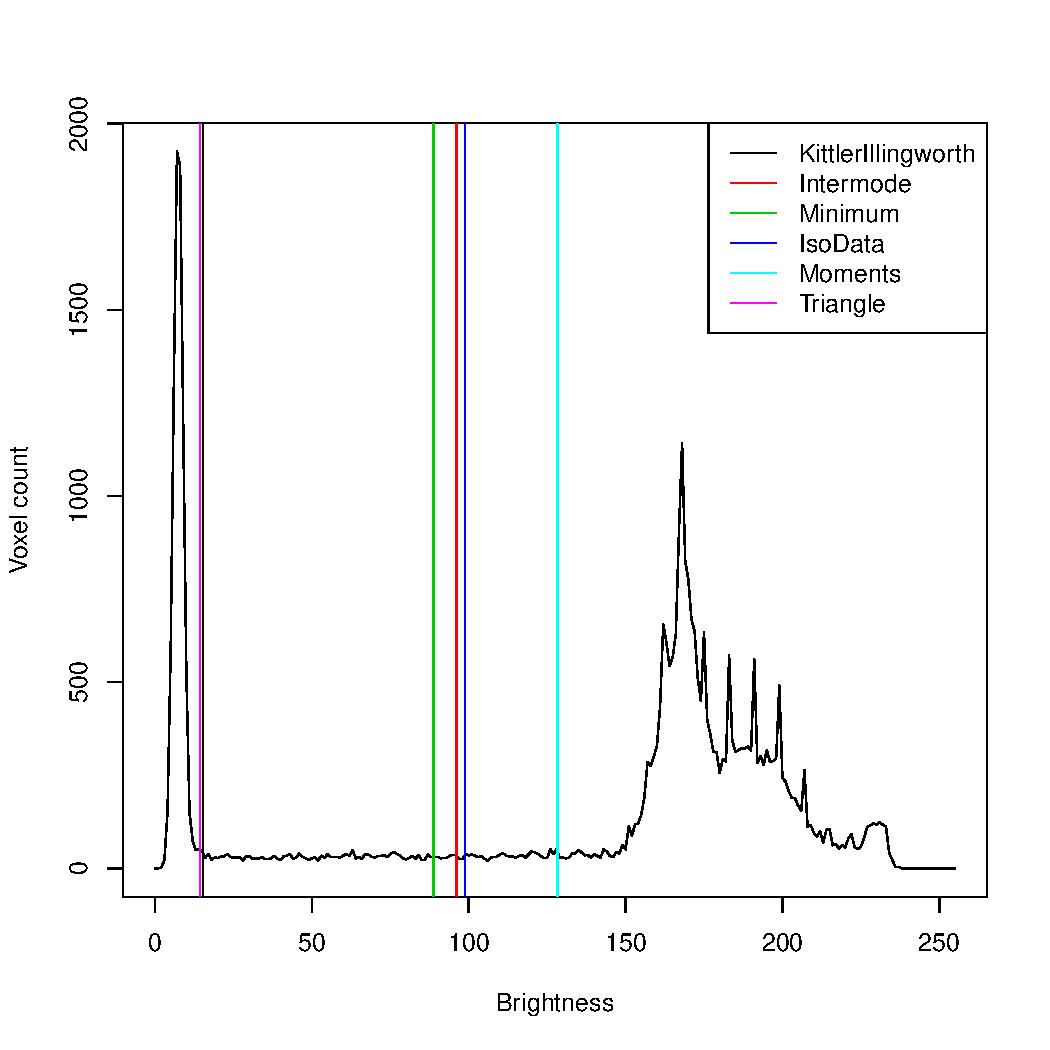
\includegraphics[height=10cm]{hist_resultsA}
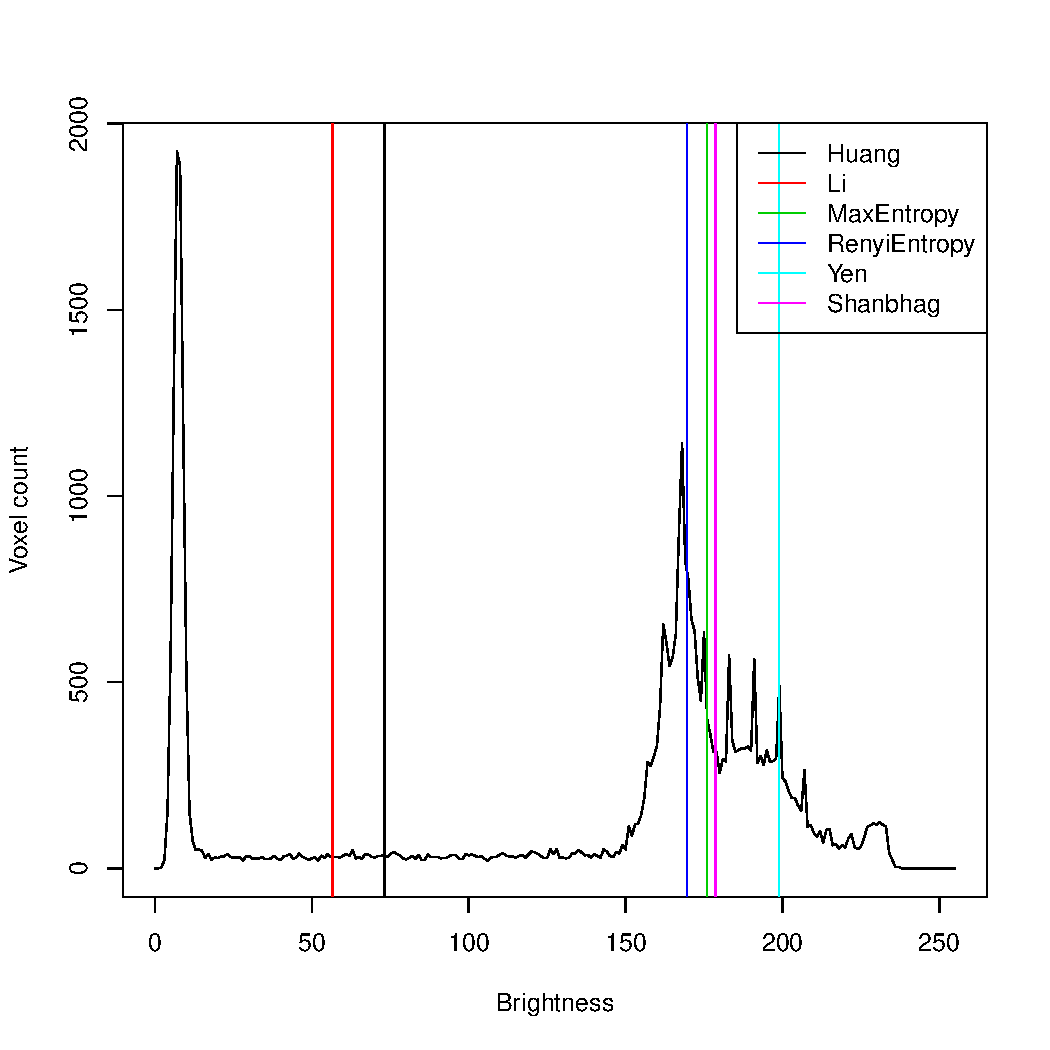
\includegraphics[height=10cm]{hist_resultsB}
\caption{Image histogram and thresholds selected by implemented methods.\label{fig:thresh}}
\end{figure}


\section{Usage}
These classes can be used in a similar way to the well-established
{\em OtsuThresholdImageFilter}. Classes are templated over input and
output image types and have methods to set the output {\em inside} and
{\em outside} pixel values, the number of histogram bins - {\em
  SetNumberOfHistogramBins}. Intermodes has a method to select the
intermodes or minimum selection option - {\em SetUseIntermodes} - and
the maximum number of smoothing iterations - {\em
  SetMaximumSmoothingIterations}.

All thresholding classes have an associated calculator class that
operates on the histogram to estimate the threshold. 

\section{Comments, conclusions and further work}
Histogram-based approaches to estimating thresholds are very useful, but also can be surprisingly sensitive to changes in image characteristics. Padding images, for example, can easily add a large spike to a histogram that can cause unexpected outputs from many methods. In the example illustrated here, changing the framing of the scene could easily change the significance of the background class leading to very different behaviour. Underlying assumptions built into some methods, such as Gaussian mixture models, can become unrealistic if image acquisition conditions (e.g. lighting) change, and such changes are not necessarily obvious to the naked eye. Always use with care and always attempt to constrain the areas to which such estimation is applied in order to minimize the chances of changes in image characteristics affecting application performance.

This contribution is a set of standard thresholding methods available in other packages. The implementation is derived from the ImageJ java plugin. These classes have been included recently in the ITK 4 distribution via Gerrit and include a variety of tests.

Several of the articles cited describe extensions to the basic methods to support multi-level thresholding. Additional control of the histogramming parameters can also be included. Only the most basic are in the current version. Finally, masked versions of these classes are also likely to be useful. This should be relatively simple to implement using the masked histogram infrastructure. Hopefully these extensions can be implemented in the future.

\appendix



\bibliographystyle{plain}
\bibliography{local}
\nocite{ITKSoftwareGuide}

\end{document}

